\RequirePackage{fix-cm}

\documentclass[twocolumn]{svjour3}          % twocolumn

\smartqed  % flush right qed marks, e.g. at end of proof
%
% \usepackage{mathptmx}      % use Times fonts if available on your TeX system
%
% insert here the call for the packages your document requires
%\usepackage{latexsym}
\usepackage{graphicx}
\usepackage{lineno,hyperref,amsmath}
\usepackage{multirow}
\usepackage[round]{natbib} 
\usepackage[misc]{ifsym}
% etc.
%
% please place your own definitions here and don't use \def but
% \newcommand{}{}
%
% Insert the name of "your journal" with
% \journalname{myjournal}
%
\begin{document}

\title{Global optimization method with dual Lipschitz constant estimates for problems with non-convex constraints\thanks{This research was supported by the Russian Science Foundation, project No. 16-11-10150.}
}

\author{Roman Strongin        \and
        Konstantin Barkalov   \and
				Semen Bevzuk
}

\institute{Roman Strongin        \and
					 Konstantin Barkalov (\Letter) \and
					 Semen Bevzuk \at
              Lobachevsky State University of Nizhni Novgorod, Nizhni Novgorod, 603950, Russia \\
              \email{konstantin.barkalov@itmm.unn.ru}
}

\date{Received: date / Accepted: date}


\maketitle

\begin{abstract}
This paper considers the constrained global optimization problems, in which the functions are of the “black box” type and satisfy the Lipschitz condition. The algorithms for solving the problems of this class require the use of adequate estimates of the a priori unknown Lipschitz constants for the problem functions. A novel approach presented in this paper is based on a simultaneous use of two estimates of the Lipschitz constant: an overestimated and an underestimated one. The upper estimate provides the global convergence whereas the lower one reduces the number of trials necessary to find the global optimizer with the required accuracy. The considered algorithm for solving the constrained problems doesn’t use the ideas of the penalty function method; each constraint of the problem is accounted for separately. The convergence conditions of the proposed algorithm are formulated in the corresponding theorem. The results of the numerical experiments on a series of multiextremal problems with non-convex constraints demonstrating the efficiency of the proposed scheme of dual Lipschitz constant estimates are presented.
\keywords{Global optimization \and Multiextremal problems \and Non-convex constraints \and Lipschitz constant estimates \and Dimensionality reduction \and Numerical methods}
%\subclass{90C26}
\end{abstract}

\section{Introduction}
\label{intro}
In this paper, we consider constrained global optimization problems and the numerical methods for solving problems of this type. Such problems are often encountered in applications (see, for example, \cite{Pinter2006}). As a rule, problem functions are defined by a program code, i.e. they are ``black-box'' functions, for which the computing of the values can be a time-consuming operation since in applied problems it will require  numerical modeling. Any  possibility to estimate reliably the global optimum in the multiextremal problems with ``black-box'' functions is based fundamentally on the auxiliary assumptions relating the possible values of the problem functions to their known values at the points of the trials already performed.
	
	The assumption that the problem functions satisfy the Lipschitz condition is typical for many applied problems (in this case, one can speak about the Lipschitzian optimization problems) because the ratio of the functions’ variations to corresponding ones of the variables usually cannot exceed some threshold determined by the limited energy of variations in the system. This threshold can be described using the Lipschitz constant.
	
	The methods for solving the Lipschitzian optimization problems constitute a very important area in the development of the global optimization methods and are the objects of investigations of many researchers. The first algorithms of this class were proposed as early as in the 1970s (\cite{Evtushenko1971,Piyavskii1972,Shubert1972,Strongin1970}); since that time, this area has been continuing to develop extensively (see, for example, \cite{Evtushenko2009,Evtushenko2013,Strongin2000,Sergeyev2013,Jones2009}). Note that these global optimization algorithms are, as a rule, oriented towards solving either  unconstrained optimization problems \break (\cite{Paulavicius2014,Sergeyev2015,Pinter1996,Jones1993,Gablonsky2001}) or problems with constraints of a simple structure (\cite{Vaz2009,Paulavicius2016}). The solving of the problems with complex non-convex constraints is usually performed with the use of the penalty functions method (\cite{Stripinis2019,Pillo2012,Pillo2016}), which has a number of drawbacks.  In particular, this method cannot be applied to the problems with the partially defined functions (i.e. when any constraint is violated, the values of all the other functions of the problem remain undefined).
	
	This situation is typical of many optimal design problems, when, in case of violation of some conditions of the modeled object's functioning, other characteristics of the object appear to be undefined. For example, the modeled object is an electronic device, and its response time is minimized. However, the response time is undefined if at a given combination of parameters the device fails to operate. Such a partial computability of the functions in the constrained optimization problems complicates essentially (in some cases, makes impossible) the application of the penalty functions method. 
	
	Within the framework of our research, an original approach to the minimization of the multiextremal functions with non-convex constraints called the index method of the accounting for the constraints  
was used (see \cite{Strongin2000,Pugliese,Barkalov2002,Strongin2003}). This approach is based on separate accounting for each constraint of the problem and does not involve the use of the penalty functions. According to the rules of the index method, every iteration called \textit{trial} at the corresponding point of the search domain includes a sequential checking of the feasibility of the problem constraints at this point. When the first violation of any constraint is found, the trial is terminated (the values of the remaining problem functions are not computed at this point) and the transition to the next iteration point is initiated. This allows solving the problems with partially defined functions. The experimental comparison of the index method of accounting for the constraints and the penalty function method demonstrated the advantages of the index method in terms of the number of iterations and the number of computations of the problem functions (\cite{Barkalov2017_1,Barkalov2017_2}).
	
	Note that the values of the Lipschitz constant for the problem functions are usually not known a priori, which  makes their estimation one of the key problems in the construction of the Lipschitzian optimization methods. The methods utilizing the values of the Lipschitz constant predefined a priori (see, for example, \cite{Piyavskii1972,Shubert1972,Wood1991,Meewella1988,Mladineo1986}) are important in the theoretical aspect, but it is difficult to use such methods in applied problems (in which the information of the Lipschitz constant values is absent).
		
		The value of the unknown Lipschitz constant estimate affects the convergence rate of the algorithm essentially. Therefore, the issue of its correct estimate is very important. An underestimate of the true value of the constant may lead to the loss of the algorithm convergence to the global solution. At the same time, too high a value of the constant estimate not corresponding to real behavior of the function results in slow convergence of the algorithm to the global minimum point. 
		
		Several typical methods for adaptive estimation of the Lipschitz constant according to the results of the performed search trials are known:
\begin{itemize}
\item global estimate of the constant $L$ in the whole search domain $D$ (\cite{Strongin2000,Pinter1996,Horst1996}).
\item local estimates of the constants $L_i$ in different subdomains $D_i$ of the search domain $D$ (\cite{Kvasov2003,Sergeyev2010,Sergeyev2016}).
\item choice of the estimates of the constant $L$ from some set of possible values (\cite{Jones2009,Jones1993,Gablonsky2001,Sergeyev2006}).
\end{itemize}

	Each of the approaches listed above has its own advantages and drawbacks. For example, the use of the global estimate only in the entire search domain may slow down the convergence of the algorithm to the global minimum point. On the other hand, the use of the local estimates accelerating the convergence requires an adequate adjustment of the algorithm parameters in order to ensure the global convergence. 

	In this paper, we consider an algorithm, in which it is proposed to use two global estimates of the Lipschitz constant, one of them being much greater than the other one. The larger estimate ensures global convergence and the smaller one reduces the total number of trials needed to find the global optimizer. The choice of one of the two estimates to be used in the rules of the algorithm is performed in the adaptive manner, depending on the behavior of the function. This work continues the research reported in \cite{NUMTA2019}, in which the preliminary results have been obtained for the unconstrained problems.
	
	The main part of the paper has the following structure. In Section \ref{sec:2}, the index method of accounting for the constraints and the dimensionality reduction scheme for the constrained global optimization problems are described. In Section \ref{sec:3}, a description of the computational rules of the index global search algorithm is given and its theoretical properties are formulated. In Section \ref{sec:4}, the index algorithm with dual Lipschitz constant estimates is formulated and its convergence is proved. Section \ref{sec:5} presents the results of the numerical experiments carried out on several series of the multiextremal problems with non-convex constraints. Section \ref{sec:6} concludes the paper.



\section{Index Method of Accounting for the Constraints and Dimensionality Reduction}
\label{sec:2}
	We consider the global optimization problems of the form
\begin{equation}\label{problem}
	\min{\left\{\varphi(y):y \in D, \; g_j(y)\leq 0, \; 1 \leq j \leq m\right\}},
\end{equation}
\begin{equation}\label{D}
	D=\left\{y\in R^N: a_i\leq y_i \leq b_i, 1\leq i \leq N\right\}.
\end{equation}

	It is supposed that the objective function $\varphi(y)$ (henceforth denoted by $g_{m+1}(y)$) and the left-hand sides $g_{j}(y)$, $1 \leq j \leq m$, of the constraints satisfy the Lipschitz condition
\begin{align}\label{lipschitz_condition}
	\left|g_j(y')-g_j (y'')\right| \leq L_j \|y'-y''\|, \nonumber \\ 
	y', y''\in D, \; 1\leq j \leq m+1,
\end{align}
with a priori unknown constants $L_j, 1\leq j \leq m+1$, and may be multiextremal.

	The analytical form of the functions $g_{j}(y)$ may be unknown, i.e. these functions may be defined algorithmically (“black-box” functions). In this case, it is supposed that even a single search trial may be a computationally costly operation since in applied problems it involves the need to perform numerical modeling. 
	
	Along with the exact solution $y^\ast$ of the problem (\ref{problem}), we will consider also the $\varepsilon$-reserved solution $y_{\epsilon}$, for which 
\small
\begin{align}\label{epsilon_reserved_solution}
	\varphi(y_{\epsilon}) = \min{\left\{\varphi(y):y \in D, g_j(y)\leq -{\epsilon}_j, 1 \leq j \leq m\right\}},
\end{align}
\normalsize
and the set of solutions $Y_{\epsilon}$, which are not worse than the $\varepsilon$-reserved solution in the objective function value, i.e.
\small
\begin{align}\label{Y_epsilon}
	Y_{\epsilon} = \left\{ y \in D, \; g_j(y) \leq 0, \; 1 \leq j \leq m, \; \varphi(y) \leq \varphi(y_{\epsilon}) \right\}.
\end{align}
\normalsize
Fig. \ref{fig:eps_reserved_solution} illustrates the concepts introduced.

\begin{figure}
	\center{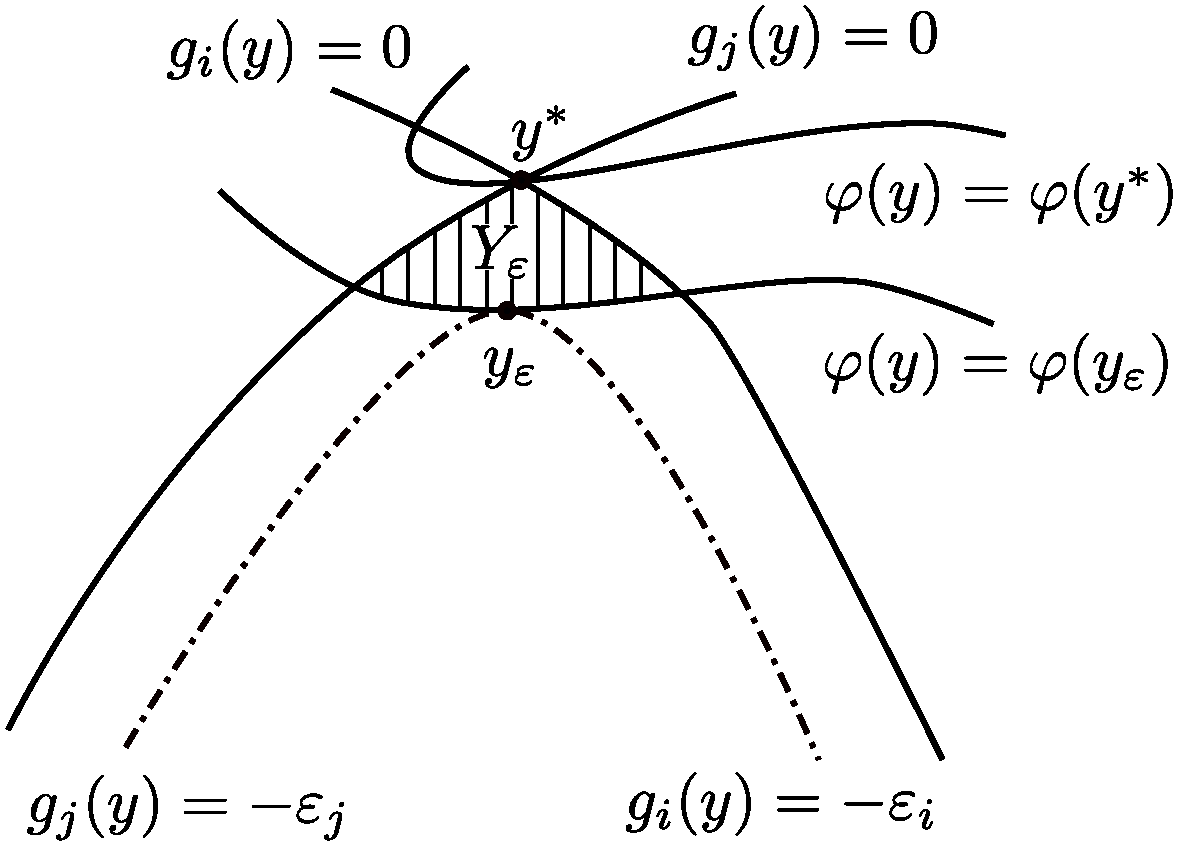
\includegraphics[width=0.6\linewidth]{Fig1}}
	\caption{$\varepsilon$-reserved solution.}
	\label{fig:eps_reserved_solution}
\end{figure}

	The existence of the $\varepsilon$-reserved solutions of problem (\ref{problem}) can be interpreted as some analog of the regularity conditions in classical nonlinear programming problems. The applied role of this condition should be also noted. Even if the exact solution $y^\ast$ is found, its practical implementation is possible as some approximation of $y^\ast$ only. Therefore, it is important that there are feasible points from $Q_{m+1}$ close enough to $y^\ast$ (in coordinates and values). The existence of the $\varepsilon$-reserved solution guarantees the existence of such points. In this case, the domain $Y_{\epsilon}$ may play the role of a set of suitable approximations.

	We will consider the initial problem (\ref{problem}) assuming that the problem functions $g_{j}(y)$, $1 \leq j \leq m+1$, may be defined only partly. It means that they are defined and computable only in the sets
\small
\begin{align}\label{D_sets}
	D_1 = D, \; D_{j+1} = \left\{ y \in D_j: \; g_j(y) \leq 0 \right\}, \; 1 \leq j \leq m.
\end{align}
\normalsize
This situation is typical for the optimal design problems when some conditions for the functioning of the modeled object are not met and its other characteristics appear to be undefined. In this approach, the first violation of any constraint indicating that the point $y$ being considered is no longer feasible terminates further computations at the point $y$.

	Many well known approaches to solving the multidimensional global optimization problems are based on either explicit or implicit reduction of multidimensional problems to one-dimensional ones (see, for example, the description of methods using the diagonal partitions in \cite{Sergeyev2006} or simplicial partitions in \cite{Zilinskas2008}). In this paper, we will use the approach based on the dimensionality reduction with the use of the space-filling curve $y(x)$ (the Peano curve). Continuous unambiguous mapping $y(x)$ projecting the interval [0,1] onto an $N$-dimensional hypercube $D$ allows reducing a multidimensional constrained minimization problem in the domain $D$ to a one-dimensional constrained optimization problem in the interval [0,1]
\small
\begin{align}\label{one_dimensional_problem}
	& \varphi(y(x^\ast)) =  \nonumber \\
	& \min \left\{\varphi(y(x)): x \in [0,1], \; g_j(y(x))\leq 0, \; 1 \leq j \leq m\right\}.
\end{align}
\normalsize
The issues of the numerical construction of the Peano space filling curve-type mappings and the corresponding theory were described in detail in \cite{Strongin2000,Sergeyev2013}. Note that the theoretical Peano curve $y(x)$ is a limit object and in practice is replaced by its approximation (called \textit{evolvent}) with predefined precision $2^{-m}$, where the number $m>1$ is a parameter (the \textit{density} of the evolvent). The evolvent density is determined by the accuracy of the possible practical implementation of the problem solution found. For  illustration, Fig. \ref{fig:evolvent} (a), (b) shows the projections of the interval [0,1] for the mapping $y(x)$ with $N=2$ and $m=4,5$, correspondingly.
\begin{figure}
	\begin{minipage}[h]{0.45\linewidth}
		\center{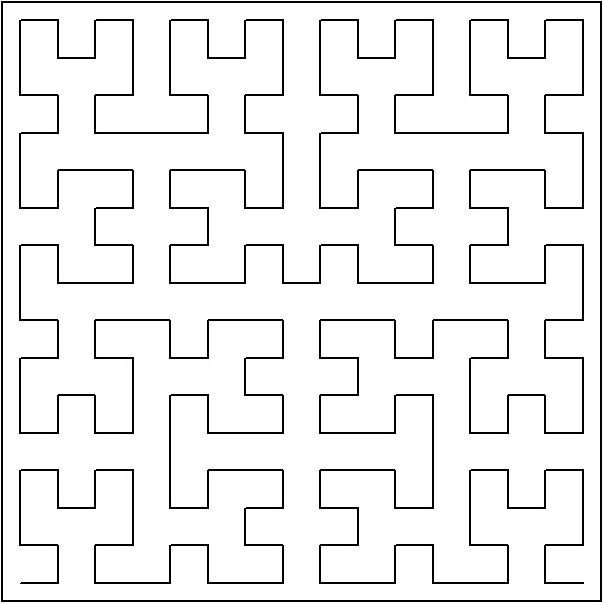
\includegraphics[width=1.0\linewidth]{Fig2} \\ {\footnotesize(a)}}
	\end{minipage}
	\hfill
	\begin{minipage}[h]{0.45\linewidth}
		\center{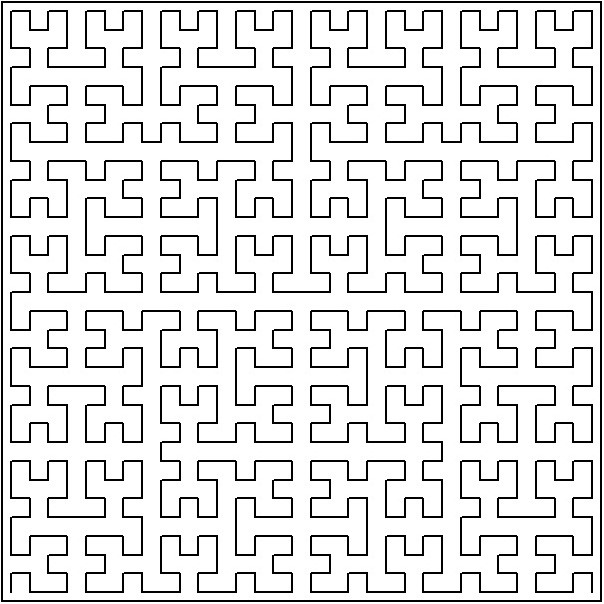
\includegraphics[width=1.0\linewidth]{Fig3} \\ {\footnotesize(b)}}
	\end{minipage}
	\caption{Evolvent for $N=2$ and $m=4$ (a), $m=5$ (b)}
	\label{fig:evolvent}
\end{figure}

	The dimensionality reduction scheme considered here matches a multidimensional problem with Lipschitzian objective function and Lipschitzian constraints to a one-dimensional problem, in which the corresponding functions satisfy the uniform H\"{o}lder condition (see \cite{Strongin2000,Sergeyev2013})
\begin{align*} 
	\left|g_j(y(x'))-g_j(y(x''))\right| \leq K_j \left|x'-x'' \right|^{1/N}, \\  
	x', x''\in [0,1], \; 1\leq j \leq m+1,
\end{align*}
where $N$ is the dimensionality of the initial multidimensional problem and the coefficients $K_j$ are related to the Lipschitz constants $L_j$ of the initial problem by the relations
\begin{equation}\label{K_leq_L}
	K_j \leq 2L_j \sqrt{N+3}, \; 1\leq j \leq m+1.
\end{equation}

	According to (\ref{D_sets}) and (\ref{one_dimensional_problem}), the reduced one-dimensional functions $g_j (y(x)), 1 \leq j \leq m+1,$ will also be defined and computable in the corresponding intervals 
\begin{align}\label{Q_intervals}
	Q_1=[0,1], \; Q_{j+1}=\left\{x \in Q_j : g_j(y(x)) \leq 0 \right\}, \nonumber \\
	1 \leq j \leq m.
\end{align}
These relations allow introducing a classification of the points $x \in [0,1]$ according to the number $\nu = \nu(x)$ of the constraints computable at the given point. We will call this number $\nu = \nu(x)$ the \textit{index} of the point $x$. The index can be determined from the conditions 
$$
	g_j(y(x)) \leq 0, \; 1 \leq j \leq \nu-1, \; g_{\nu}(y(x))>0,
$$
where the last inequality is insufficient if $\nu = m+1$. 

	Thus, a search trial at some point $x^k \in [0,1]$ performed at the $k^{th}$ iteration of the algorithm will consist of the following sequence of operations:
\begin{itemize} 
  \item determine the image $y^k=y(x^k )$ with the use of the evolvent $y(x)$. 
  \item compute the values $g_1 (y^k ), \ldots ,g_{\nu} (y^k )$, where $\nu = \nu(x^k)$ is the index of the point $x^k$.
	\item fix the result of the trial as three values 
\begin{equation}\label{trial_result}
	x^k, \; z^k = g_{\nu}\left( y(x^k) \right), \; \nu = \nu(x^k).
\end{equation}
\end{itemize}
	
	According to this scheme, the trial is terminated at the point $y^k=y(x^k)$ when the first violated constraint  is found.
	
	In the case when the point $y^k = y(x^k)$ is a feasible one, i.e. when $x^k \in Q_{m+1}$, the trial involves checking all constraints and computing the objective function. Here, the value of the index $\nu$ is accepted to be equal to $m+1$.
	
	The main idea of the index scheme of accounting for the constraints consists in the reduction of the constrained problem (\ref{one_dimensional_problem}) (the functions of which satisfy the H\"{o}lder condition with corresponding coefficients $K_j$) to an unconstrained problem of the form
\begin{equation}\label{reduction_problem}
	\psi(x^*)=\min \left\{\psi(x): x \in [0,1] \right\},
\end{equation}
\begin{eqnarray*}
	\psi(x)=\frac{g_{\nu}(y(x))}{K_{\nu}} - 
	\left\{
   \begin{array}{lr}
     0, & \nu \leq m,\\
     \frac{\varphi^\ast}{K_{m+1}}, & \nu = m + 1,
   \end{array}
	\right.
\end{eqnarray*}
where $\nu = \nu(x)$ and $\varphi^\ast$ is the objective function value at the point of the problem solution (\ref{one_dimensional_problem}).

	The value $\psi(x)$ at $\nu(x) \leq m$ matches the value of the left-hand side of the first constraint violated at this point $g_{\nu}(y(x))$ divided by the constant $K_{\nu}$. In the case when $\nu(x) = m+1$ 
$$
	\psi(x)=\frac{\varphi(y(x))-\varphi^\ast}{K_{m+1}}
$$
and, consequently, the set of the points, in which the function $\psi(x)$ turns to zero matches the set of the global minimum points of the problem (\ref{one_dimensional_problem}). It should be noted that in any subdomain $Q_j$ the function $\psi(x)$ has the H\"{o}lder coefficient equal to 1.
	
	These considerations constitute the basis of the index global search algorithm, according to which the unknown constants $K_{\nu}$ and the unknown minimum value $\varphi^\ast$ are substituted in the course of computations by their current approximations.



\section{Index-Based Global Search Algorithm}
\label{sec:3}
	The index-based global search algorithm under consideration for solving the problem (\ref{problem}) (here it is given according to \cite{Strongin2000}) involves the construction of a sequence of points $x^k \in (0,1)$, at which the search trials are conducted with the results of the type (\ref{trial_result}). The set of triplets 
$\{x^k,\; z^k=g_{\nu}\big(y(x^k)\big),\; \nu=\nu(x^k)\},\; 1 \leq k \leq n,$
makes up the search information accumulated by the method after performing $n$ steps. The operation of the index-based global search algorithm is defined by the following rules.
	
	The first trial is executed at an arbitrary internal point $x^1 \in (0,1)$. The selection of the point $ x^{k+1}, k \geq 1$, of any next trial is determined by the following steps. \\
Step 1. Renumber the points $x^1, \ldots, x^k$ of the preceding trials by the lower indices in the increasing order of the coordinate values, i.e.
$$
	0=x_0<x_1<\dots <x_k<x_{k+1}=1,
$$
and juxtapose to them the values $z_i=g_{\nu}\big(y(x_i)\big),\nu=\nu(x_i), 1 \leq i \leq k$, computed at these points. The points $x_0=0$ and $x_{k+1}=1$ are introduced additionally and the values $z_0$ and $z_{k+1}$ are not defined. \\
Step 2. Classify the indices $i, 1 \leq i \leq k$, of the trial points in accordance with the number of the constraints of the problem fulfilled at these points by constructing the sets
$$
	I_\nu =\left\{i:1 \leq i \leq k, \; \nu=\nu(x_i) \right\}, \; 1 \leq \nu \leq m+1,
$$
including the numbers of all points $x_i, 1 \leq i \leq k,$ with the same values of $\nu$. The end points $x_0=0$ and $x_{k+1}=1$ are interpreted as the ones having the indices equal to zero. An additional set $I_0=\{0, k+1\}$ corresponds to these points.

	Determine the maximum value of the index 
$$
	M=\max\left\{\nu=\nu(x_i), \; 1 \leq i \leq k \right \}.
$$ \\
Step 3. Compute the current lower bounds
\begin{equation}\label{current_lower_bounds}
	\mu_{\nu} = \max\left\{ \frac{\left|z_i-z_j\right|}{ (x_i - x_j)^{1/N} }, \; i,j \in I_\nu, \; i>j \right\}
\end{equation}
for the unknown H\"{o}lder constants $K_{\nu}$ of the functions $g_{\nu}, 1 \leq \nu \leq m+1$. If the set $I_{\nu}$ includes less than two elements or if $\mu_{\nu}$ appears to be equal to zero, then set $\mu_{\nu}=1$. \\
Step 4. For all nonempty sets $I_{\nu}, 1 \leq \nu \leq m+1$, compute the estimates
\begin{equation}\label{z_estimates}
	z_\nu^\ast = \left\{
   \begin{array}{lr}
     -\epsilon_\nu, & \nu < M,\\
     \min\{ z_i: i\in I_\nu \}, & \nu = M,
   \end{array}
	\right.
\end{equation}
where the nonnegative numbers $(\epsilon_1,\ldots,\epsilon_m )$ are the algorithm parameters. \\
Step 5. For each interval $(x_{i-1}, x_i), 1 \leq i \leq k+1$, compute the \textit{characteristics} $R(i)$:
\begin{align}\label{R_1}
	R(i)=\Delta_i+\frac{(z_i-z_{i-1})^2}{r_\nu^2 \mu_\nu^2\Delta_i}-2\frac{z_i+z_{i-1}-2z_\nu^\ast}{r_\nu \mu_\nu}, \nonumber \\ 
 \nu=\nu(x_i)=\nu(x_{i-1}),
\end{align}
\begin{equation}\label{R_2}
	R(i)=2\Delta_i-4\frac{z_i-z_\nu^\ast}{r_\nu \mu_\nu}, \; \nu=\nu(x_i)>\nu(x_{i-1}),
\end{equation}
\begin{equation}\label{R_3}
R(i)=2\Delta_i-4\frac{z_{i-1}-z_\nu^\ast}{r_\nu \mu_\nu}, \; \nu=\nu(x_{i-1})>\nu(x_i),
\end{equation}
where $\Delta_i=(x_i-x_{i-1})^{1/N}$. The values $r_{\nu} > 1, 1 \leq \nu \leq m+1$, are the parameters of the algorithm. With an appropriate selection of $r_{\nu}$ one can use the product $r_{\nu}\mu_{\nu}$ as an estimate of H\"{o}lder constants $K_{\nu}, 1 \leq \nu \leq m+1$. \\
Step 6. Find the interval $(x_{t-1}, x_t)$ with the maximum characteristic
\begin{equation}\label{MaxR}
	R(t)=\max{\left\{R(i): 1 \leq i \leq k+1\right\}}.
\end{equation} 
Step 7. Execute the next trial at the middle point of the interval $(x_{t-1}, x_t)$ if the indices of the points $x_{t-1}, x_t$ are not the same, i.e.,
$$
	x^{k+1} = \frac{x_t + x_{t-1}}{2}, \; \nu(x_{t-1}) \neq \nu(x_t).
$$
Otherwise, execute a trial at the point
\begin{align*}
	x^{k+1} = \frac{x_t+x_{t-1}}{2} + \frac{\mathrm{sign}(z_t-z_{t-1})}{2r_\nu}\left[\frac{\left|z_t-z_{t-1}\right|}{\mu_\nu}\right]^N, \; \\
	\nu=\nu(x_{t-1})=\nu(x_t).
\end{align*}
The inequality $\Delta_t \leq \epsilon$ can be taken as the termination condition, where $t$ is from (\ref{MaxR}) and $\epsilon>0$ is the predefined accuracy.

	The convergence conditions for the index global search algorithm can be formulated in the form of the following theorem from \cite{Strongin2000}. 
\\
\begin{theorem}\label{theorem:1} Assume that the following conditions are satisfied:
	\begin{enumerate} 
		\item Problem (\ref{problem}) has an $\varepsilon$-reserved solution $y_{\varepsilon}$ from (\ref{epsilon_reserved_solution}).
		\item Functions $g_j(y), 1 \leq j \leq m+1,$ admit Lipschitzian (with the constants $L_j$) extensions $G_{j}(y)$ over the whole feasible domain $D$ from (\ref{D}), i.e.
	$$
		g_j \left( y(x) \right) = G_j \left( y(x) \right), \; x \in Q_j, \; 1 \leq j \leq m+1,
	$$
	where the sets $Q_j$ are from (\ref{Q_intervals}), and $y(x)$ is the curve from (\ref{one_dimensional_problem}).
		\item The parameters of the method $\epsilon_{\nu}, 1 \leq \nu \leq m,$ used in the rule (\ref{z_estimates}) are the corresponding components of the reserve vector $\epsilon_{R}$ from (\ref{epsilon_reserved_solution}).
		\item For a sufficiently large iteration number $k$, the values $\mu_{\nu}$ from (\ref{current_lower_bounds}) satisfy the inequalities
			\begin{equation}\label{theorem_inequalities}
				r_{\nu}\mu_{\nu} > 2^{3-\frac{1}{N}}L_{\nu}\sqrt{N+3}, \; 1 \leq \nu \leq m+1. 
			\end{equation}
	\end{enumerate}
	Then, any limit point $\bar{y}$ of the sequence of the trials $\{y^k\}=\big\{y\big(x^k\big)\big\}$ generated by the index algorithm for problem (\ref{problem}) belongs to the set $Y_{\epsilon}$ from (\ref{Y_epsilon}) and satisfies the conditions
	\begin{eqnarray*}
		\varphi(\bar y) & = &	\inf\left\{\varphi(y^k):g_j(y^k) \leq 0, 1 \leq j \leq m, k = 1,2,\ldots \right\} \\
		& \leq & \varphi(y_{\epsilon}).
	\end{eqnarray*}
\end{theorem}
\textbf{Note 1}. The computational scheme of the algorithm is described in the form convenient for  formulating its theoretical properties. The software implementation of this scheme may be made more frugal. For example, according to Step 7, the point $x^{k+1}$ of the next trial will be an internal point of the interval $(x_{t-1}, x_t)$, i.e. $x^{k+1} \in (x_{t-1}, x_t)$. Therefore, the set of trial points $x^1,\ldots, x^k$ (and the related trial results (\ref{trial_result})) may not be ordered  at every step of the algorithm but may be maintained in an ordered state using appropriate data structures.
\\
\textbf{Note 2}. The use of the set of parameters $\epsilon_1,\ldots,\epsilon_m$ (the values of which correspond to the coordinates of the reserve vector $\epsilon_R$) in the index algorithm will significantly reduce the density of the trial sequence in the vicinity of the feasible domain boundaries. However, this raises a question about the particular values of the reserve vector components $\epsilon_R$. In \cite{Strongin2000}, it was proposed to choose the components of the vector $\epsilon_R$ according to the formula 
\begin{equation}\label{epsilon_nu}
	\epsilon_{\nu} = \mu_{\nu}\delta, \; 1 \leq \nu \leq m, 
\end{equation}
where $\mu_{\nu}$ are the current estimates from (\ref{current_lower_bounds}) and $\delta>0$ is a parameter. This approach to choosing the reserve vector components allows one to take into account the properties of different problem functions characterized by their Lipschitz constants. This method for choosing the reserve vector was used in the numerical experiments, the results of which are presented below.
\\
\textbf{Note 3}. The index algorithm for solving the constrained problems is based on the information-statistical algorithm of global search (AGS) for solving unconstrained problems. AGS has been compared repeatedly with both deterministic and nature-inspired global optimization algorithms. The results of the experimental comparison (see, for example, \cite{Sovrasov2019}) show that AGS is superior to many known methods of similar purpose, including DIRECT and DIRECT\textit{l}.

	At the same time, the index scheme of accounting for the constraints also demonstrated its advantages (in the number of computed values of the problem functions) over the traditional penalty functions method in solving a wide range of test problems (see the results of the experimental comparison in \cite{Barkalov2017_1,Barkalov2017_2}.)



\section{Index Algorithm with Dual Lipschitz Constant Estimates}
\label{sec:4}
	The index global search algorithm described in the previous section (hereafter referred to as IA) is intended for solving  the multiextremal problems, in which the objective function and the constraints satisfy the Lipschitz condition.  In this case, a priori estimates of the constant values are not required for the algorithm to work. These estimates are computed in the course of global search, based on the available search information. 
	
	According to Theorem \ref{theorem:1}, the sequence of trial points $\{y^k\}$ will converge to a point $\bar y \in Y_\epsilon$ if the condition (\ref{theorem_inequalities}) is satisfied. So far, an appropriate choice of the parameters $r_{\nu}$ allows using the values
\begin{equation}\label{estimates_Lipschitz_constants}
	\frac{r_{\nu}\mu_{\nu}}{2^{3-\frac{1}{N}}\sqrt{N+3}}, \; 1 \leq \nu \leq m+1, 
\end{equation}
as the estimates of the Lipschitz constants for the problem functions $g_{j}(y), 1 \leq j \leq m+1$.

	Compliance with condition (\ref{theorem_inequalities}) will be achieved when choosing a high values of the parameters $r_{\nu}$. However, in this case the constant will be overestimated, and the method will perform a large number of trials until the stopping condition is fulfilled.
	The choice of low values of the parameters $r_{\nu}$ (which corresponds to an underestimate of the Lipschitz constant) would reduce the number of trials considerably but could destroy the convergence to the global extremum (due to possible violation of the condition (\ref{theorem_inequalities})).
	
	An approach, in which two estimates of the Lipschitz constant for each function are used in the rules of the algorithm, is promising. One of these estimates is significantly greater than the other, which corresponds to the use of two sets of parameters $r_{\nu}^{glob}$ and $r_{\nu}^{loc}$ in the algorithm, where $r_{\nu}^{glob}>r_{\nu}^{loc}>1, 1 \leq \nu \leq m+1$. When using the parameter $r_{\nu}^{loc}$ we shall deal with the smaller estimate of the Lipschitz constant, and using the parameter $r_{\nu}^{glob}$ will correspond to the larger one.
	
	We will refer to the characteristics of the $i^{th}$ interval as the global ones $(R_{glob}(i))$ if the parameters $r_{\nu}=r_{\nu}^{glob}$ were used when computing the characteristic according to (\ref{R_1}), (\ref{R_2}), (\ref{R_3}) and as the local ones  $(R_{loc}(i))$ if the parameters $r_{\nu}=r_{\nu}^{loc}$ were used. 

	The key idea of the novel method is computing two characteristics for each interval and balancing (based on these two) the local and global search. The local search provides a new trial in the vicinity of the current minimum point $y_k^\ast$  whereas during the global search a new trial could be performed in a subdomain located far away from $y_k^\ast$. 
	
	Note that Theorem \ref{theorem:1} on the convergence of the index method implies the generation of an infinite sequence of trials $\{y^k\}=\big\{y(x^k )\big\}$ by the algorithm. In this case, at the final stage of the search (i.e. in the case when one of the points of this trial sequence falls into the vicinity of the $\varepsilon$-reserved solution $y_\epsilon$) there always exists an interval, at one of the boundaries of which the current minimum value of the objective function $z_{m+1}^\ast$  from (\ref{z_estimates}) is achieved. It is this interval that will have the highest characteristic since it is the most promising one for performing further trials. 

	Let us establish the following important property for the global and local characteristics of an interval containing the current minimum point.

	\textbf{Statement}. Let us assume that the current minimum value $z_M^\ast$  from (\ref{z_estimates}) at the $k^{th}$ iteration is achieved at the boundary point of some interval $[x_{i-1}, x_i], i=i(k)$. Then, $R_{glob}(i) \geq R_{loc}(i)$.

	\textbf{Proof}. Let us consider two possible cases of the values of the indices $\nu(x_{i-1})$ and $\nu(x_i)$. 
\begin{enumerate} 
  \item If $\nu(x_{i-1}) \neq \nu(x_i)$, then according to  formulae (\ref{R_2}), (\ref{R_3}) 
\begin{equation}\label{R_glob_1}
	R(i)=R_{glob}(i)=R_{loc}(i)=2\Delta_i>0. 
\end{equation}
  \item If $\nu(x_{i-1}) = \nu(x_i) = M$, then, taking into account (\ref{current_lower_bounds}), the following inequality will hold
$$
	z_i+z_{i-1}-2z_M^* = |z_i-z_{i-1}|\leq \mu_M\Delta_i .
$$
\end{enumerate} 
From here, it will follow that for any value $r_M>1$ the following inequalities will hold
\begin{align}
	R(i) & = \Delta_i + \frac{(z_i-z_{i-1})^2}{r_M^2\mu_M^2\Delta_i} - 2\frac{z_i+z_{i-1}-2z_M^*}{r_M\mu_M} \geq \nonumber \\
	& \geq  \Delta_i + \frac{(z_i-z_{i-1})^2}{r_M^2\mu_M^2\Delta_i} - 2\frac{\mu_M\Delta_i}{r_M\mu_M} \geq \nonumber \\
  & \geq \Delta_i + \frac{(z_i-z_{i-1})^2}{r_M^2\mu_M^2\Delta_i} - 2\frac{\Delta_i}{r_M} = \nonumber \\
	& = \Delta_i + \Delta_i\frac{(z_i-z_{i-1})^2/\Delta_i^2}{r_M^2\mu_M^2\Delta_i^2} - 2\frac{\Delta_i}{r_M} \geq \nonumber \\
	& \geq \Delta_i + \frac{\Delta_i}{r_M^2} - 2\frac{\Delta_i}{r_M} = \Delta_i \left( 1-\frac{1}{r_M} \right)^2>0.
\end{align}
And because $r_{M}^{glob} > r_{M}^{loc} > 1$, then
\begin{align}\label{R_glob_greater_R_loc}
	R_{glob}(i) & = \Delta_i\left(1-\frac{1}{r_M^{glob}} \right)^2 > \nonumber \\
	& > \Delta_i\left(1-\frac{1}{r_M^{loc}} \right)^2 = R_{loc}(i).
\end{align}
The statement is proved.

	This statement can be interpreted as the incomparability of the local and global characteristics: the global characteristic of the best interval is always larger. At the same time, it follows from the formulae (\ref{R_glob_1}), (\ref{R_glob_greater_R_loc}) that 
\begin{equation}\label{R_glob_equal_R_loc}
	R_{glob}(i) = \rho R_{loc}(i),
\end{equation}
where $\rho=\Big(\frac{1-1/r_{M}^{glob}}{1-1/r_{M}^{loc}}\Big)^2$, if $\nu(x_{i-1})=\nu(x_i)=M$, and $\rho=1$, if $\nu(x_{i-1}) \neq \nu(x_i)$. In the case of the multiplication by the coefficient $\rho$, the local and global characteristics of the search intervals become comparable, and one can choose the best (i.e. the largest) one.

	Based on the relation (\ref{R_glob_equal_R_loc}), one can formulate an \textit{index algorithm with dual estimate of the Lipschitz constants} (hereafter referred to as IA-DL).
	
	The first four steps of the algorithm repeat Step 1 -- Step 4 of the initial index algorithm from Section \ref{sec:3}.
	
	Step 5. For each interval $(x_{i-1}, x_i), 1 \leq i \leq k+1$: 
\begin{flushleft}
	\begin{itemize}
		\item compute the global characteristics $R_{glob}(i)$ according to formulae (\ref{R_1}), (\ref{R_2}), (\ref{R_3}) using the value $r_{\nu}=r_{\nu}^{glob}$;
		\item compute the local characteristics $R_{loc}(i)$ according to formulae (\ref{R_1}), (\ref{R_2}), (\ref{R_3}) using the value $r_{\nu}=r_{\nu}^{loc}$;
		\item determine the characteristic $R(i)$ as
\begin{equation}\label{R_max}
	R(i) = \max{\left\{ R_{glob}(i), \rho R_{loc}(i) \right\}},
\end{equation}
where $\rho=\Big(\frac{1-1/r_{\nu}^{glob}}{1-1/r_{\nu}^{loc}}\Big)^2$ if $\nu(x_{i-1})=\nu(x_i)=\nu$, and $\rho=1$ if $\nu(x_{i-1}) \neq \nu(x_i)$.
	\end{itemize}
\end{flushleft}

	Step 6. Find the interval $(x_{t-1}, x_t)$ with the maximum characteristic
\begin{equation}\label{R_max_t}
	R(t) = \max{\left\{ R(i): 1 \leq i \leq k+1\right\}}
\end{equation}
and fix the value $r_{\nu}=r_{\nu}^{loc}$ if $\rho R_{loc}(t) > R_{glob}(t)$, otherwise fix $r_{\nu}=r_{\nu}^{glob}$.

	Step 7. Execute the next trial at the middle point of the interval $(x_{t-1}, x_t)$ if the indices of the points $x_{t-1}$, $x_t$ are not the same, i.e.
$$
	x^{k+1} = \frac{x_t + x_{t-1}}{2}, \; \nu(x_{t-1}) \neq \nu(x_t).
$$
Otherwise, execute a trial at the point
\begin{eqnarray*}
	x^{k+1} = \frac{x_t+x_{t-1}}{2} + \frac{\mathrm{sign}(z_t-z_{t-1})}{2r_\nu}\left[\frac{\left|z_t-z_{t-1}\right|}{\mu_\nu}\right]^N, \\
	\nu = \nu(x_{t-1})=\nu(x_t).
\end{eqnarray*}
When computing the point $x^{k+1}$, use the value of the parameter $r_{\nu}$ fixed at Step~6. 

The algorithm terminates if the condition $\Delta_{t} \leq \epsilon$ is satisfied where $t$ is from (\ref{R_max_t}) and $\epsilon>0$ is the predefined accuracy.

	Let us illustrate the work of the algorithms IA and IA-DL when minimizing the function
\small
\begin{align*}
	&\varphi(y_1, y_2) = -1.5y_1^2\exp{\left\{1-y_1^2-20.25(y_1-y_2)^2\right\}}-\\
	& -\left(0.5(y_1-1)(y_2-1)\right)^4 \exp{\left\{2-\left(0.5(y_1-1)\right)^4-(y_2-1)^4\right\}}
\end{align*}
\normalsize
in the range $0 \leq y_1 \leq 4$, $1 \leq y_2 \leq 3$ subject to the constraints
\small
\begin{eqnarray*}
	g_1(y_1, y_2) & = & 0.01 \left( (y_1-2.2)^2+(y_2-1.2)^2-2.25 \right) \leq 0, \\
	g_2(y_1, y_2) & = & 100 \left(1-(y_1-2)^2/1.44+(0.5y_2)^2 \right) \leq 0, \\
	g_3(y_1, y_2) & = & 10 \left( y_2 - 1.5 - 1.5 \sin{\left( 6.283(y_1-1.75) \right)}\right) \leq 0.
\end{eqnarray*}
\normalsize
The feasible domain of this problem is non-connected and consists of three subdomains. The global minimum $\varphi(y^\ast)=-1.489$ is achieved at the point \\ $y^\ast =(0.942, 0.944)$ (the values are given with the accuracy of $10^{-3}$).

\begin{figure}[h]
	\begin{minipage}[h]{0.48\linewidth}
		\center{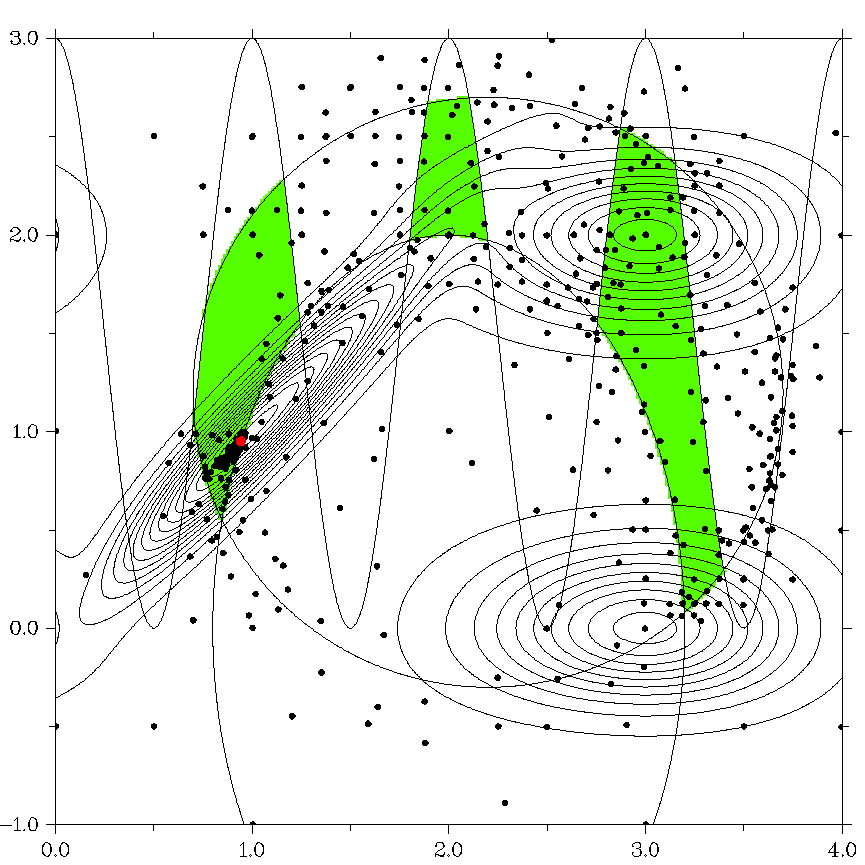
\includegraphics[width=\linewidth]{Fig4} \\ {\footnotesize(a)}}
	\end{minipage}
	\hfill
	\begin{minipage}[h]{0.48\linewidth}
		\center{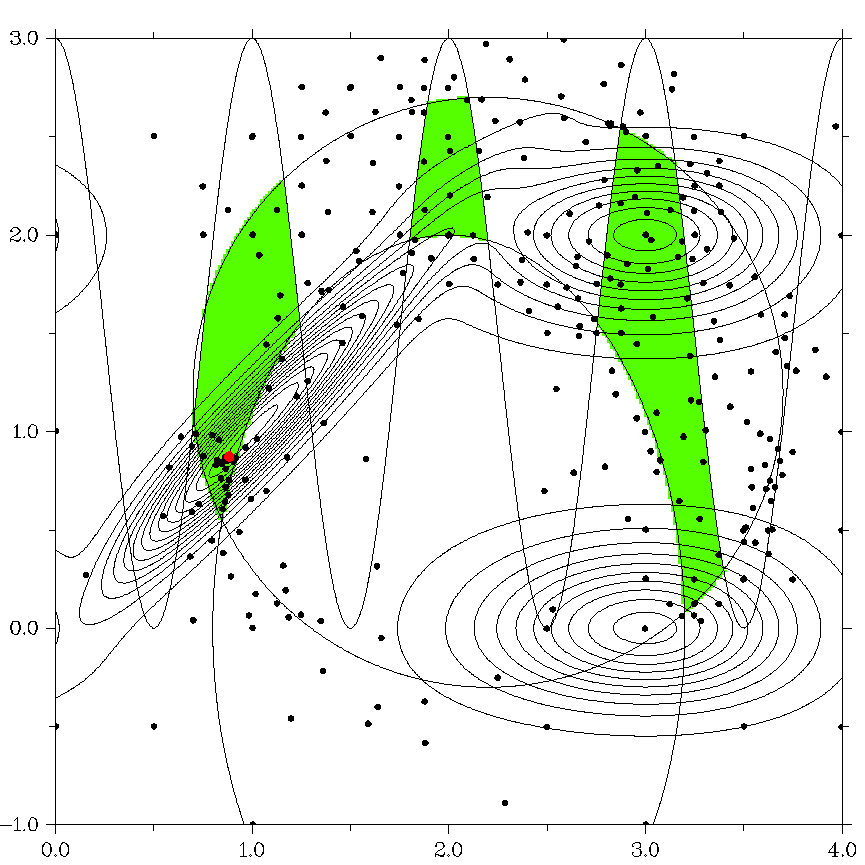
\includegraphics[width=\linewidth]{Fig5} \\ {\footnotesize(b)}}
	\end{minipage}
	\caption{Solving a problem by IA (a) and IA-DL (b) methods}
	\label{fig:example_strongin}
\end{figure}

	In Fig. \ref{fig:example_strongin}, the search domain (square) is shown, the feasible domain is highlighted by green, and the trial points generated by IA (a) and IA-DL (b) are marked. The best point is marked by red. For both methods, the evolvent with the parameter $m=10$ was used, the accuracy of the search for the solution $\epsilon=0.002$; the adaptive reserve parameter $\delta=0.008$ from (\ref{epsilon_nu}). For the IA method, the parameters $r_{\nu}=2.3, 1 \leq \nu \leq 4$, were used. The same values were used for the IA-DL method as the parameters $r_{\nu}^{glob}, 1 \leq \nu \leq 4$. Also, the parameters $r_{\nu}^{loc}=1.5, 1 \leq \nu \leq 4,$ were used. To solve the problem with a predefined accuracy $\epsilon=0.002$, 478 trials were required for the IA method compared to only 303 trials for the IA-DL method. The results of larger-scale numerical experiments are presented in Section \ref{sec:4}.

	Let us formulate and prove the convergence conditions for the new algorithm IA-DL.\\
\begin{theorem}\label{theorem:2} Let us assume the index algorithm (IA) is applied to solve the problem (\ref{problem}) and for the values $r_{\nu}=r_{\nu}^{glob}, 1 \leq \nu \leq m+1,$ the conditions of Theorem \ref{theorem:1} are fulfilled. Then, the algorithm with dual estimate of the Lipschitz constants (IA-DL) with the parameters $r_{\nu}^{glob}>r_{\nu}^{loc}>1,\; 1\leq \nu \leq m+1,$ when solving the same problem also generates a sequence of the trial points $\{y^k\}=\{y(x^k)\}$, any limit point $\bar{y}$ of which belongs to the set $Y_{\epsilon}$ from (\ref{Q_intervals}), i.e. satisfies the condition 
\begin{align}\label{phi_bar_y}
	\varphi(\bar y) & = \inf\left\{\varphi(y^k):g_j(y^k) \leq 0, 1 \leq j \leq m, k = 1,2,\ldots \right\} \nonumber \\
	& \leq \varphi(y_{\epsilon}).
\end{align}
\end{theorem}

\textbf{Proof}. Because for the IA with the parameters $r_{\nu}=r_{\nu}^{glob}, 1 \leq \nu \leq m+1,$ the conditions of Theorem \ref{theorem:1} are fulfilled, then any limit point $\bar{y}=y(\bar{x})$ of the trial sequence generated by the IA for the problem (\ref{problem}) satisfies the conditions (\ref{phi_bar_y}).

	Let us show that $\bar y$ is also the limit point of the sequence of trials $\{y^k\}=\{y(x^k)\}$, generated by the IA-DL, and the sequence $\{y^k\}$ has no new limit points. Let us carry out the proof by contradiction. Assume that $\bar y$ is not a limit point of the sequence $\{y^k\}$ and there exists a limit point $y' \neq \bar y$.

	At every iteration of the IA-DL method there will exist such interval $[x_{j-1}, x_j]$, $j=j(k)$, that $\bar x \in [x_{j-1}, x_j]$. According to our assumption that $\bar y = y(\bar x)$ is not the limit point, there will exist such number $k$, starting from which the trial points will not fall into the interval $[x_{j-1}, x_j]$. That is, to conduct a new trial at the point $x^{k+1} \in [x_{t-1}, x_t]$ at every iteration such interval $[x_{t-1}, x_t], t=t(k)$ will be selected that $t \neq j$.

	Therefore, in the formula (\ref{R_max}) for computing the characteristic, the second component takes the highest values, i.e. $ R_{glob}(t) < \rho R_{loc}(t)$.
Then, there will exist a limit point $x' \neq \bar x$, at that either $\nu(x') \leq m$ (i.e. the point $y(x')$ is not a feasible one) or $z_{m+1}^\ast =g_{m+1}(y(x'))>g_{m+1}(y(\bar x))$ (i.e. the value of the objective function at the limit point $y(x')$ is greater than at the point $y(\bar x)$).

	Let us show that if the conditions of Theorem \ref{theorem:1} are satisfied, the inequality $R_{glob}(j)>0$ will hold. According to the second condition of Theorem \ref{theorem:1} and to the condition (\ref{K_leq_L}), 
\begin{align}
	& z_j = g_{\nu}\left( y(x_j) \right) \leq g_{\nu}\left( y(\bar x) \right) + 2L_{\nu}\sqrt{N+3}(x_j-\bar x)^{1/N}, \nonumber \\
	& \nu = \nu(x_j),
\end{align}
\begin{align}
	z_{j-1} & = g_{\nu}\left( y(x_{j-1}) \right) \leq \nonumber \\
	& \leq g_{\nu}\left( y(\bar x) \right) + 2L_{\nu}\sqrt{N+3}(\bar x - x_{j-1})^{1/N}, \nonumber \\
	& \nu = \nu(x_{j-1}).
\end{align}

	Since the point $\bar y = y(\bar x)$ belongs to the set $Y_{\epsilon}$, then
\begin{equation*}
	g_{\nu}\left( y(\bar x) \right) \leq -\epsilon_{\nu}, \; 1\leq\nu\leq m,
\end{equation*}
\begin{equation*}
	g_{m+1}\left( y(\bar x) \right) \leq z_{m+1}^\ast.
\end{equation*}

	Then, the characteristic $R_{glob}(j)$ of the interval \break
$[x_{j-1}, x_j]$, $j=j(k)$ will be strictly positive, i.e. \break
$R_{glob}(j)>0$. Indeed, at $\nu=\nu(x_j)=\nu(x_{j-1})$ and the value $r_{\nu}=r_{\nu}^{glob}$
\small
\begin{align*}
	& R(j) = \Delta_i + \frac{(z_j-z_{j-1})^2}{r_{\nu}^2\mu_{\nu}^2\Delta_i} - 2\frac{z_j+z_{j-1}-2z_{\nu}^{\ast}}{r_{\nu}\mu_{\nu}} \geq \Delta_i + \\ 
	& + 4\frac{z_{\nu}^*-\left( g_{\nu}\left( y(\bar x) \right)+L_{\nu}\sqrt{N+3}\left( (x_j-\bar x)^{\frac{1}{N}}+(\bar x - x_{j-1})^{\frac{1}{N}} \right)\right)}{r_{\nu}\mu_{\nu}}\\
	& = \Delta_i-4\frac{L_{\nu}\sqrt{N+3}\left( (x_j-\bar x)^{\frac{1}{N}}+(\bar x - x_{j-1})^{\frac{1}{N}} \right)}{r_{\nu}\mu_{\nu}} + \\
	& + 4\frac{z_{\nu}^\ast-g_{\nu}\left( y(\bar x) \right)}{r_{\nu}\mu_{\nu}} \geq \\
	& \geq \Delta_i\left(1-4\frac{L_{\nu}\sqrt{N+3}\max_{0\leq\alpha\leq1} {\left( \alpha^{\frac{1}{N}}+(1-\alpha)^{\frac{1}{N}} \right)}}{r_{\nu}\mu_{\nu}} \right) + \\
	& + 4\frac{z_{\nu}^{\ast}-g_{\nu}\left( y(\bar x) \right)}{r_{\nu}\mu_{\nu}} = \\
	& = \Delta_i\left(1-4\frac{2^{3-1/N}L_{\nu}\sqrt{N+3}}{r_{\nu}\mu_{\nu}} \right)+4\frac{z_{\nu}^{\ast}-g_{\nu}\left( y(\bar x) \right)}{r_{\nu}\mu_{\nu}} > 0.
\end{align*}
\normalsize
At $\nu=\nu(x_j ) > \nu(x_{j-1})$ and the value $r_{\nu}=r_{\nu}^{glob}$
\begin{align*}
	& R(j) = 2\Delta_i - 4\frac{z_j-z_{\nu}^{\ast}}{r_{\nu}\mu_{\nu}} \geq \\
	& \geq 2\Delta_i+4\frac{z_{\nu}^{\ast}-\left( g_{\nu}\left(y(\bar x)\right)+2L_{\nu}\sqrt{N+3}(x_j-\bar x)^{\frac{1}{N}} \right)}{r_{\nu}\mu_{\nu}} = \\
	& = 2\Delta_i - 8\frac{L_{\nu}\sqrt{N+3}(x_j-\bar x)^{\frac{1}{N}}}{r_{\nu}\mu_{\nu}}+4\frac{z_{\nu}^{\ast}-g_{\nu}\left( y(\bar x) \right)}{r_{\nu}\mu_{\nu}} \geq \\
	& \geq 2\Delta_i\left( 1-4\frac{L_{\nu}\sqrt{N+3}}{r_{\nu}\mu_{\nu}} \right) + 4\frac{z_{\nu}^{\ast}-g_{\nu}\left( y(\bar x) \right)}{r_{\nu}\mu_{\nu}} > 0.
\end{align*}

	The case of $\nu=\nu(x_{j-1})>\nu(x_j)$ is treated similarly and leads to the same inequality $R(j)>0$.

	Since we have assumed that $x'$ is a limit point for the IM-DL and  $x' \neq \bar x$, then there exists such a sequence of the intervals $[x_{t-1}, x_t], t=t(k)$ that $x' \in [x_{t-1}, x_t], R_{loc}(t)>0$, and $R_{loc}(t) \rightarrow 0$. This property of the characteristics of the intervals shrinking to the limit point has been established when proving the theorem on the convergence of the IA in \cite{Strongin2000}.

	Therefore, for large enough, the following inequality will be true
\begin{equation}
	R_{glob}(j) > \rho R_{loc}(t)
\end{equation}
and (according to Rules 5 and 6 of the IA-DL method) the next iteration falls into the interval $[x_{j-1}, x_j]$, which contradicts our assumption regarding the non-limit nature of the point $\bar x$. The theorem is proven.



\section{Numerical experiments}
\label{sec:5}
To demonstrate the efficiency of the proposed algorithm, let us consider the results of solving several series of multidimensional constrained global optimization problems. In order to construct the problems, the functions generated by the GKLS generator (\cite{Gaviano2003}) were used. This generator of multiextremal functions is often used for investigating global optimization algorithms (\cite{Sergeyev2015,Paulavicius2014,Barkalov2018}). According to \cite{Gaviano2003}, we used simpler and more complex functions, which are  further denoted as ``Simple'' and ``Hard'', respectively. The complexity of the functions is determined, in particular, by the radius of the global minimizer's attraction region and by the distance between global and local minimizers.
	
	In \cite{Gergel2017_2,Gergel2019}, an approach was proposed that allows constructing the constrained global optimization problems using certain classes of multiextremal functions (in particular, the GKLS functions), in which:
\begin{itemize}
  \item the number of constraints can be varied;
  \item the volume of the feasible subdomain $Q_{m+1}$ relative to the whole search domain $D$ is defined;
	\item the global minimizer is known in advance and can be located at the boundary of the feasible domain;
	\item the number of constraints active in the global minimizer can be predefined.
\end{itemize}	

	In the experiments that we have conducted, the number of constraints in the problems was equal to 2, and one of these constraints was active at the point of the global minimum. For example, the level lines of the objective functions and constraints for $N=2$ are presented in Figs. \ref{fig:examples_simple} and \ref{fig:examples_hard}; the feasible domains are highlighted by green. It can be seen that the feasible domains in these problems are non-convex and non-connected, and the global minimizers are located at the boundaries of the feasible domains. Also, one can see that the problems of the ``Hard'' class have, in general, a more complex structure: the global minimizers are located at the boundaries of the feasible domains of smaller areas whereas in the problems of the ``Simple'' class the optimizers are located at the boundaries of the subdomains of greater areas.
	
\begin{figure}[h!]
	\begin{minipage}[h]{0.48\linewidth}
		\center{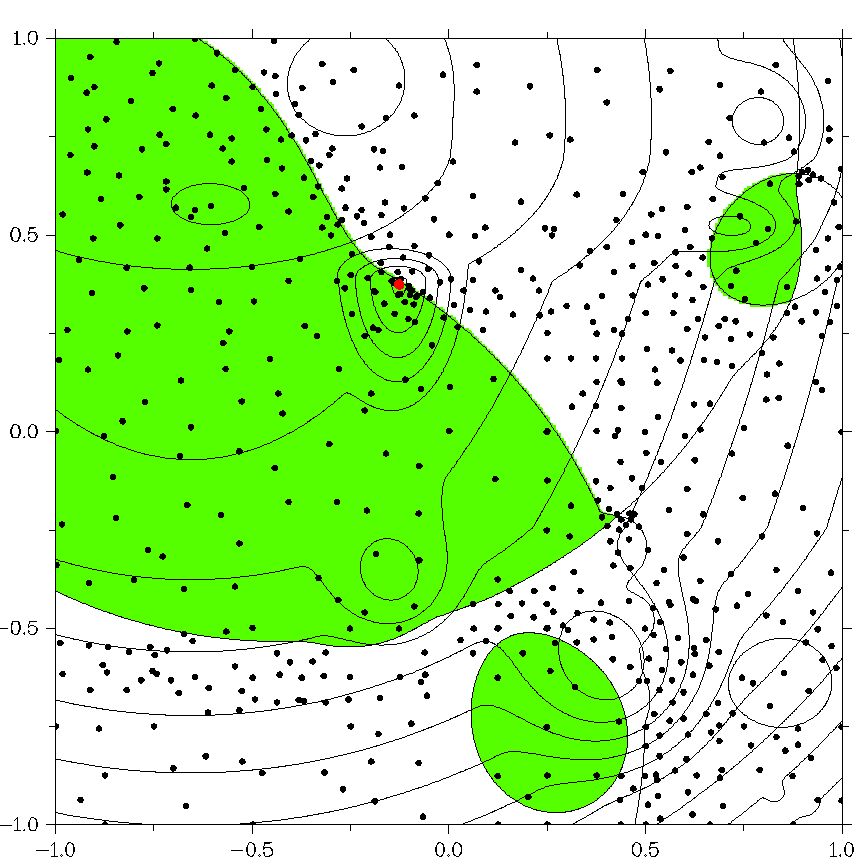
\includegraphics[width=\linewidth]{Fig6} \\ {\footnotesize(a)}}
	\end{minipage}
	\hfill
	\begin{minipage}[h]{0.48\linewidth}
		\center{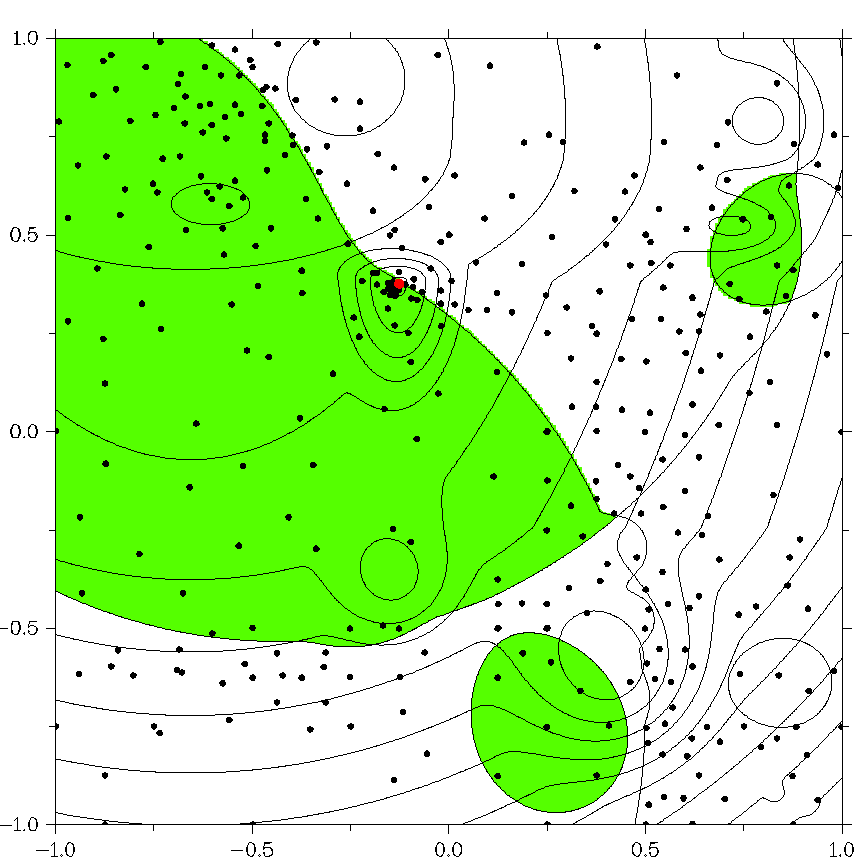
\includegraphics[width=\linewidth]{Fig7} \\ {\footnotesize(b)}}
	\end{minipage}
	\caption{Solving a problem of the “Simple” class by IA (a) and IA-DL (b) methods}
	\label{fig:examples_simple}
\end{figure}

\begin{figure}[h!]
	\begin{minipage}[h]{0.48\linewidth}
		\center{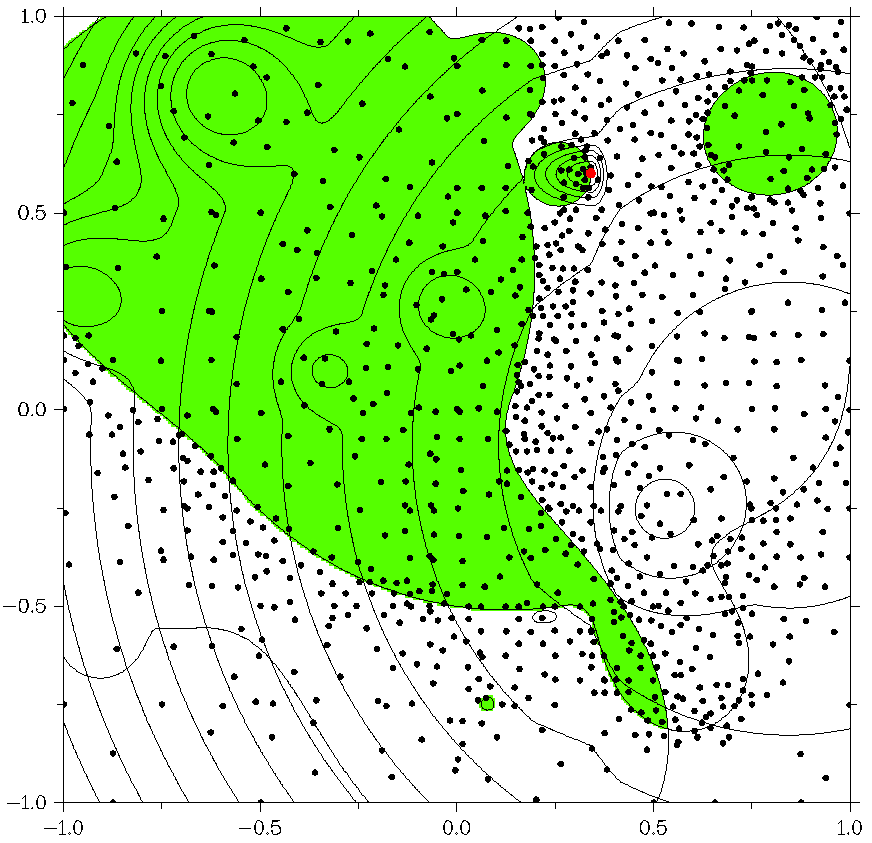
\includegraphics[width=\linewidth]{Fig8} \\ {\footnotesize(a)}}
	\end{minipage}
	\hfill
	\begin{minipage}[h]{0.48\linewidth}
		\center{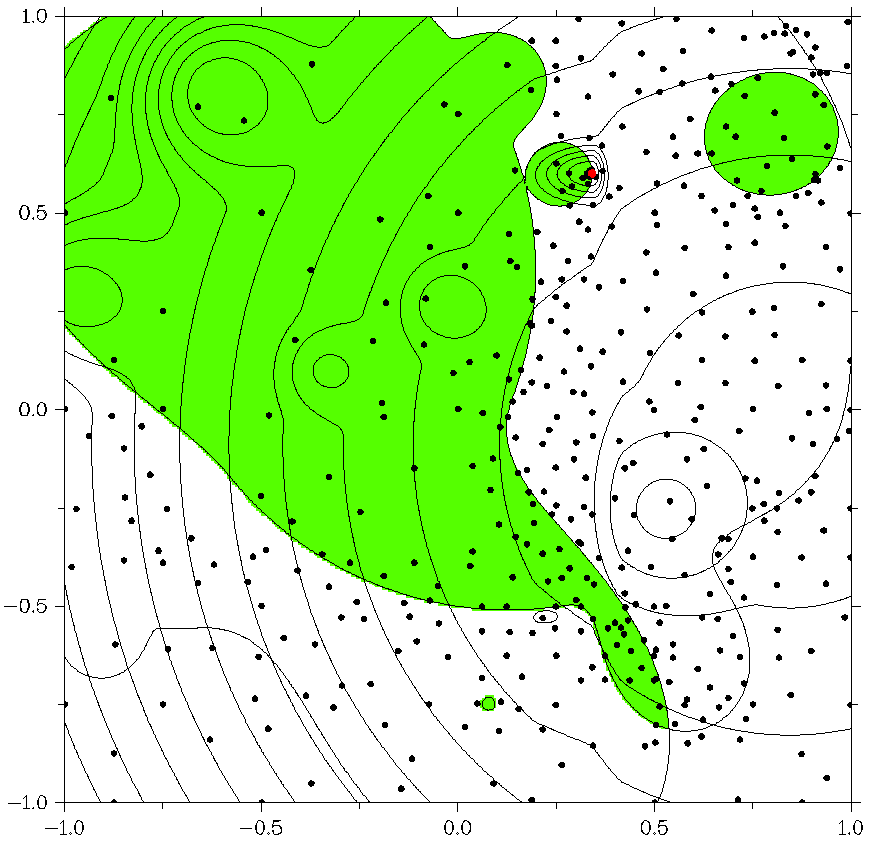
\includegraphics[width=\linewidth]{Fig9} \\ {\footnotesize(b)}}
	\end{minipage}
	\caption{Solving a problem of the “Hard” class by IA (a) and IA-DL (b) methods}
	\label{fig:examples_hard}
\end{figure}

	Also, the points of the trials performed by (a) the original index algorithm (IA) and by (b) the method with dual estimate of the Lipschitz constant (IA-DL) are marked in Figs. \ref{fig:examples_simple} and \ref{fig:examples_hard}. To solve the problems shown in Figs. \ref{fig:examples_simple} and \ref{fig:examples_hard}, the IA method required 643 and 1132 iterations whereas the IA-DL method solved similar problems for 373 and 443 iterations, respectively.
	
	The reduction of the number of trials was also confirmed by solving several series of  problems composed of the functions of the “Simple” and “Hard” classes. Each series consisted of 100 problems and was solved by the IA and IA-DL methods. The global minimizer $y^{\ast}$ was considered to be found, if the algorithm generated a trial point $y^k$ in the vicinity of the global minimum, i.e. $\| y^{\ast} - y^k \| < \varepsilon \|b - a\|$, where $a$ and $b$ are the boundaries of the search domain $D$. To reduce the dimensionality, the evolvent constructed with the parameter $m=10$ was used in both algorithms. The relative accuracy of the search for the solution at $N = 2, 3$ was $\epsilon=0.01$ and for the solution at $N=4,5$  it was $\epsilon=0.03$. The reservation parameters $\epsilon_{\nu}=\mu_{\nu} \delta,\; 1 \leq \nu \leq 2$, were set according to formula (\ref{epsilon_nu}) with $\delta=0.01$. The maximum number of iterations at $N \leq 4$ was set as $K_{max} = 10^6$, and at $N=5$ as $K_{max}=7 \cdot 10^6$.

	Since all functions involved in the statement of each particular problem belong to the same class, equal parameters $r_{\nu}=4.1$ were set for the problems of the “Simple” class and $r_{\nu}=6.2$ for the problems of the “Hard” class. When solving the problems of these classes by the IA-DL method, the values of the parameters $r_{\nu}$ given above were selected for the upper estimate of the Lipschitz constants, i.e. the values $r_{\nu}^{glob}=4.1$ and $r_{\nu}^{glob}=6.2$ were set, which were supplemented by various values of $r_{\nu}^{loc}$. The average number of iterations performed by the algorithms with different values of $r_{\nu}^{loc}$ is given in Table \ref{tab:average_number_of_iterations_simple} and \ref{tab:average_number_of_iterations_hard}. The number of unsolved problems is given in brackets.

\begin{table}[h!]
	\caption{Average number of iterations performed by the methods on “Simple” class}
	\label{tab:average_number_of_iterations_simple}
	\begin{tabular}[]{ccccc}
		\hline\noalign{\smallskip}
		                    & $N=2$                & $N=3$                    & $N=4$                  & $N=5$                   \\
		\noalign{\smallskip}\hline\noalign{\smallskip}
		IA-DL,              & \multirow{2}{*}{316} & \multirow{2}{*}{7403}    & \multirow{2}{*}{40419} & \multirow{2}{*}{296357} \\
		$r_{\nu}^{loc}=1.4$ &                      &                          &                        &                         \\
		\noalign{\smallskip}
		IA-DL,              & \multirow{2}{*}{350} & \multirow{2}{*}{8990(1)} & \multirow{2}{*}{41230} & \multirow{2}{*}{360497} \\
		$r_{\nu}^{loc}=2.0$ &                      &                          &                        &                         \\
		\noalign{\smallskip}
		IA                  & 439                  & 11804(1)                 & 41973(3)               & 404660(2)               \\
		\hline\noalign{\smallskip}
	\end{tabular}
\end{table}

\begin{table}[h!]
	\caption{Average number of iterations performed by the methods on “Hard” class}
	\label{tab:average_number_of_iterations_hard}
	\begin{tabular}{ccccc}
		\hline\noalign{\smallskip}
		                    & $N=2$                & $N=3$                    & $N=4$                  & $N=5$                      \\
		\noalign{\smallskip}\hline\noalign{\smallskip}
		IA-DL,              & \multirow{2}{*}{766} & \multirow{2}{*}{9636}    & \multirow{2}{*}{60904} & \multirow{2}{*}{763711}    \\
		$r_{\nu}^{loc}=1.4$ &                      &                          &                        &                            \\
		\noalign{\smallskip}
		IA-DL,              & \multirow{2}{*}{830} & \multirow{2}{*}{12020}   & \multirow{2}{*}{57473} & \multirow{2}{*}{743874(1)} \\
		$r_{\nu}^{loc}=2.0$ &                      &                          &                        &                            \\
		\noalign{\smallskip}
		IA                  & 1074                 & 20327                    & 87310(2)               & 1084990(2)                 \\
		\hline\noalign{\smallskip}
	\end{tabular}
\end{table}

	In addition to the average number of trials required to solve the problems, the results of solving the series of problems can be also presented by the function $p(k)$, which describes the number of problems solved for $k$ iterations. This function will be called the \textit{operational characteristic} of the algorithms.
	
	The operational characteristics for IA and IA-DL obtained by solving the series of problems of the “Simple” and “Hard” classes with the dimensionalities $N=3$ and $N=5$ are presented in Figs. \ref{fig:operational_characteristics_N=3} and \ref{fig:operational_characteristics_N=5}, respectively. The values of parameters $r_{\nu}$ used to evaluate the Lipschitz constant are given in the figures.

\begin{figure}[h!]
	\begin{minipage}[h]{0.48\linewidth}
		\center{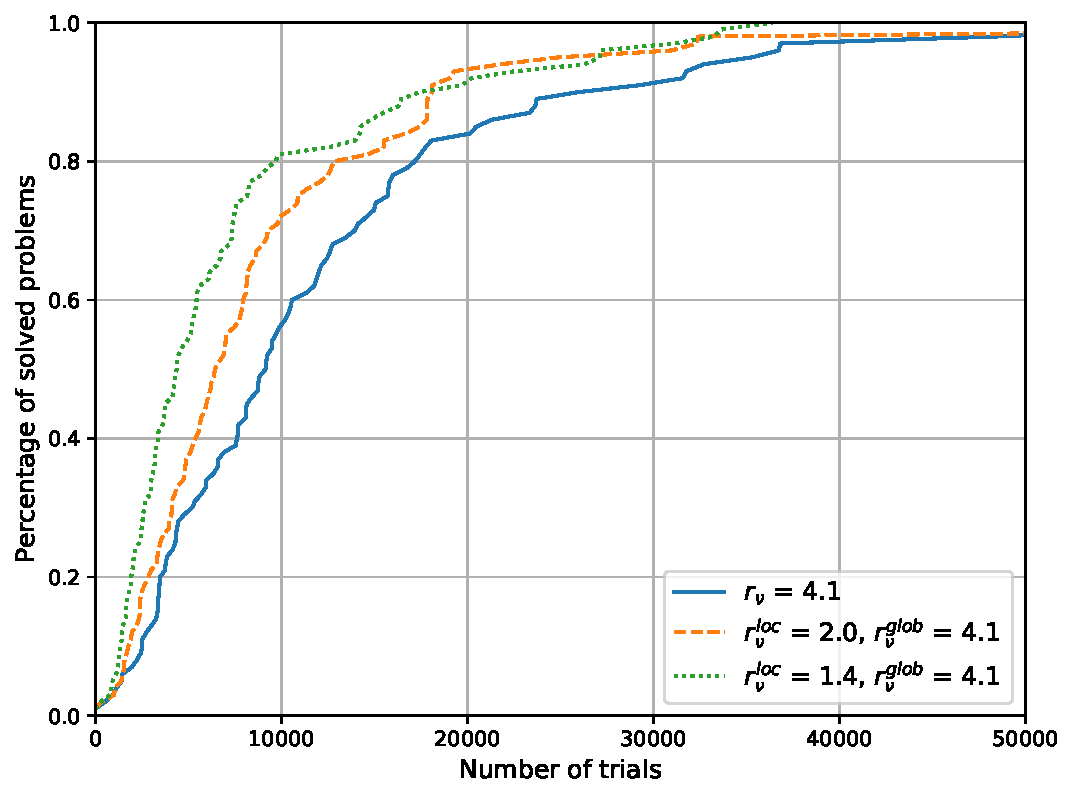
\includegraphics[width=\linewidth]{Fig10} \\ {\footnotesize(a)}}
	\end{minipage}
	\hfill
	\begin{minipage}[h]{0.48\linewidth}
		\center{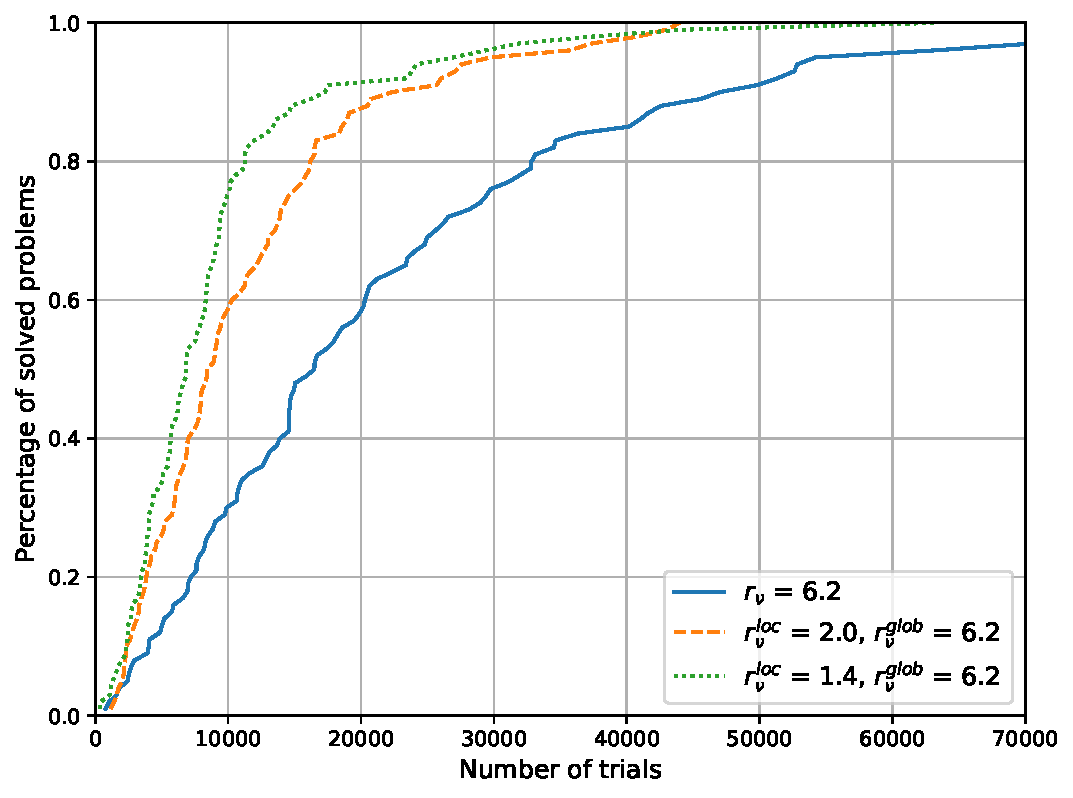
\includegraphics[width=\linewidth]{Fig11} \\ {\footnotesize(b)}}
	\end{minipage}
	\caption{Operational characteristics for “Simple” (a) and “Hard” (b) problem classes, $N = 3$}
	\label{fig:operational_characteristics_N=3}
\end{figure}

\begin{figure}[h!]
	\begin{minipage}[h]{0.48\linewidth}
		\center{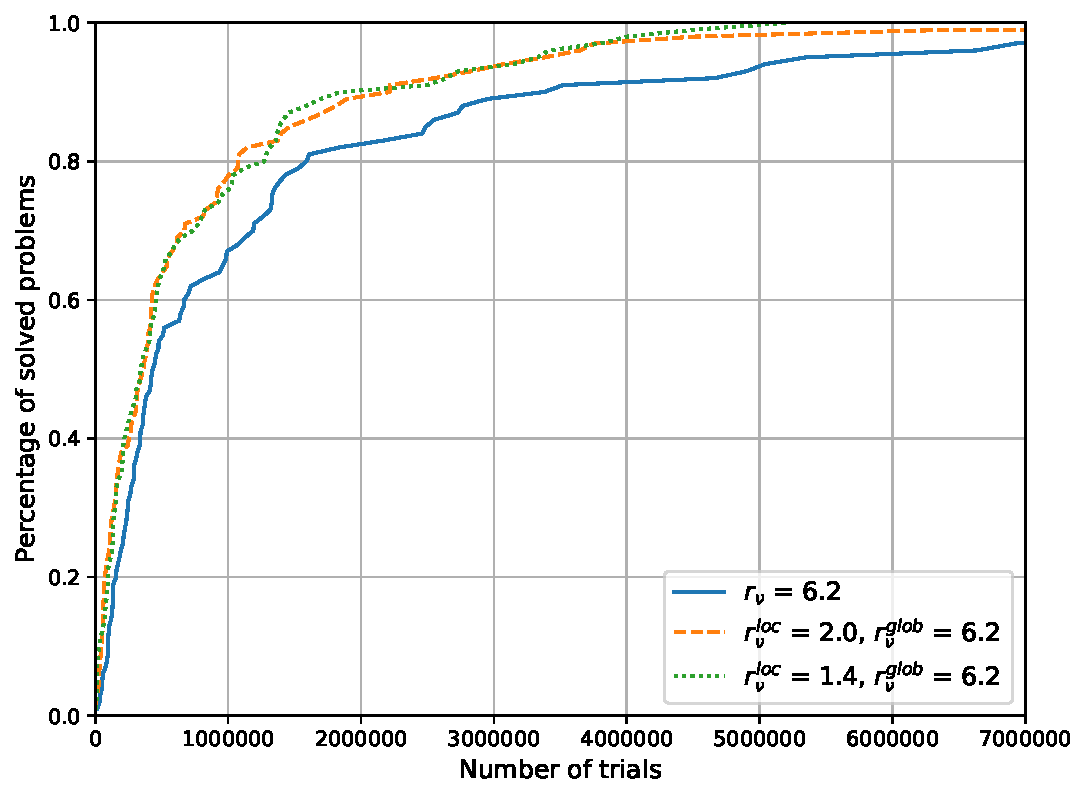
\includegraphics[width=\linewidth]{Fig12} \\ {\footnotesize(a)}}
	\end{minipage}
	\hfill
	\begin{minipage}[h]{0.48\linewidth}
		\center{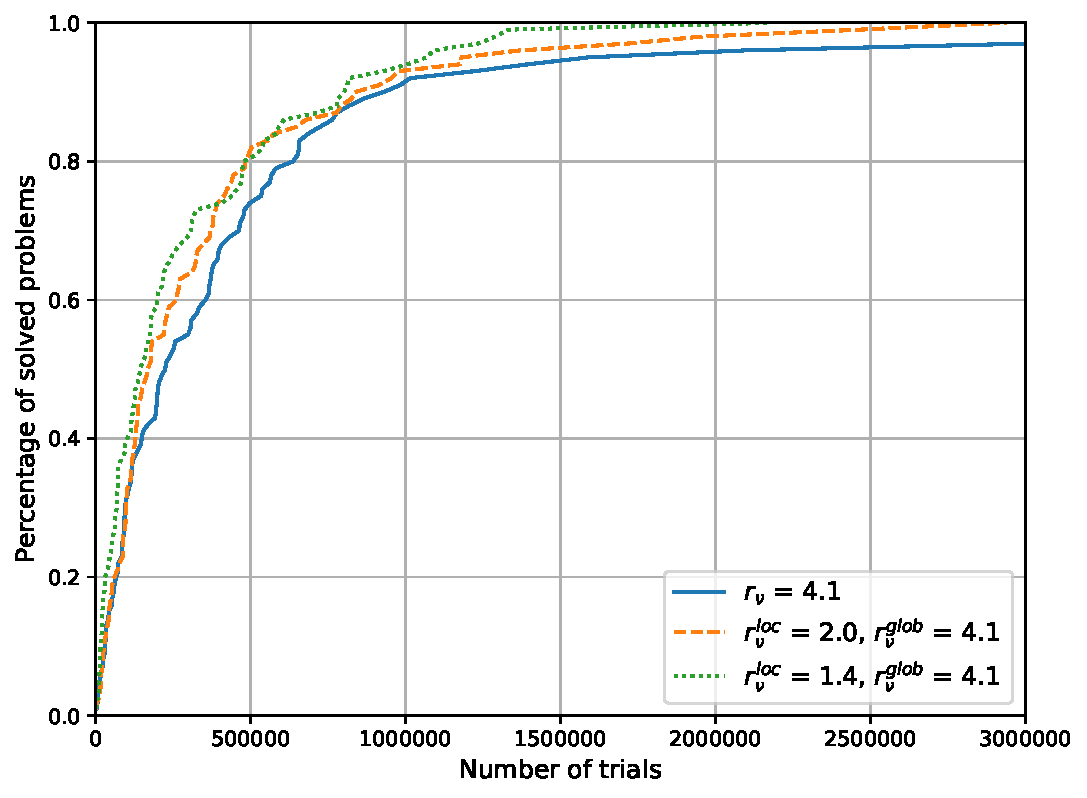
\includegraphics[width=\linewidth]{Fig13} \\ {\footnotesize(b)}}
	\end{minipage}
	\caption{Operational characteristics for “Simple” (a) and “Hard” (b) problem classes, $N = 5$}
	\label{fig:operational_characteristics_N=5}
\end{figure}

	The lower (solid) curves in Figs. \ref{fig:operational_characteristics_N=3} and \ref{fig:operational_characteristics_N=5} characterize IA whereas the upper (dashed) lines characterize IA-DL. This arrangement of curves shows that the algorithm with dual estimates of the Lipschitz constant  provides, on average, a faster solution to the problems of the series than the algorithm using a single estimate of the Lipschitz constant.
	
	The frequency of the use of the upper and lower estimates of the Lipschitz constant in the rules of the algorithm that corresponds to the choice of $r_{\nu}=r_{\nu}^{loc}$ or $r_{\nu}=r_{\nu}^{glob}$ according to Step 6 of the algorithm is an interesting indicator. This frequency can be characterized by the average values $K_{glob}$ and $K_{loc}$ of the use of the respective (global or local) characteristic. In order to present this frequency, let us plot the number of trials normalized from 1 to 100 on the abscissa axis. Actually, in this case the abscissa axis will reflect the progress in solving the problem (in percentage) where 1 corresponds to the beginning and 100 -- to the end of the process of the search for the solution. The indicators $K_{glob}$ and $K_{loc}$ will be plotted on the ordinate axis. Such plots are presented in Fig. \ref{fig:frequency_N=4}.

\begin{figure}[h!]
	\begin{minipage}[h]{0.48\linewidth}
		\center{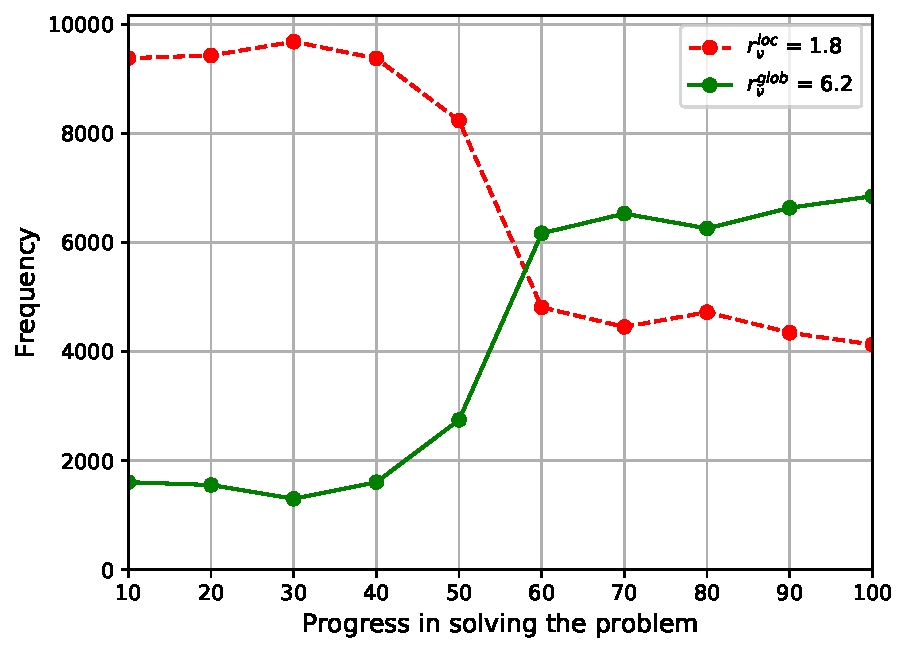
\includegraphics[width=\linewidth]{Fig14} \\ {\footnotesize(a)}}
	\end{minipage}
	\hfill
	\begin{minipage}[h]{0.48\linewidth}
		\center{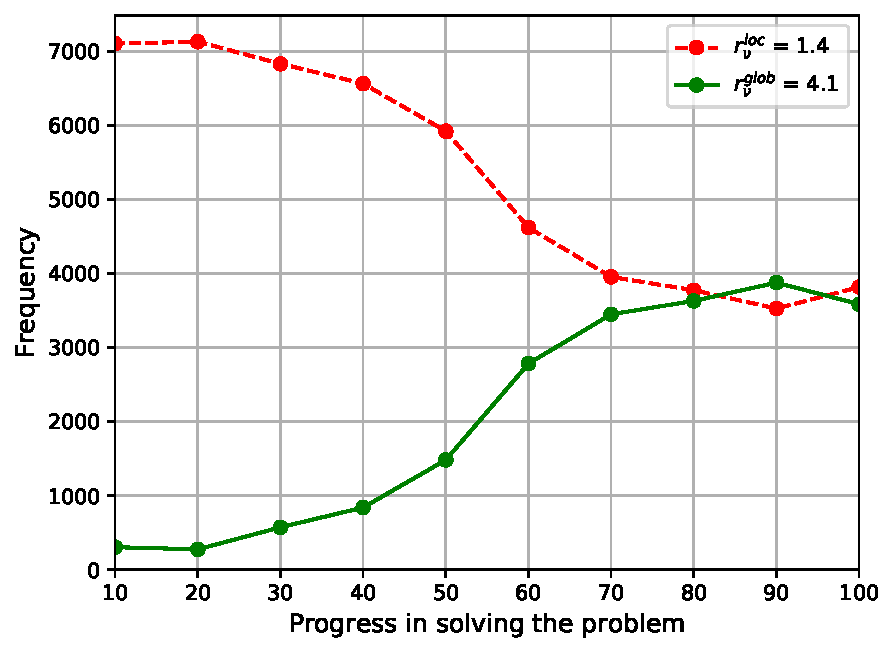
\includegraphics[width=\linewidth]{Fig15} \\ {\footnotesize(b)}}
	\end{minipage}
	\caption{Frequency of the use of different estimates of the Lipschitz constant for the problems of the “Simple” class (a) and of the “Hard” class (b) for $N=4$}
	\label{fig:frequency_N=4}
\end{figure}

	The dashed lines in Fig. \ref{fig:frequency_N=4} correspond to the frequency of the use of the lower estimates of the Lipschitz constant, the solid lines -- to the frequency of the use of the upper estimate. The arrangement of the curves shows the lower estimate of the Lipschitz constant to be used more frequently  at the beginning of the search process whereas at the final stage both estimates are used with almost equal frequency. These plots coincide qualitatively with the frequencies of the use of different estimates of the Lipschitz constant for other series of problems as well.



\section{Conclusion}
\label{sec:6}
	In this paper, a method for solving the Lipschitz optimization problems, which constitute an important class of the global optimization problems, was considered. In applied global optimization problems, the functions are usually defined as the “black boxes”. Consequently, the values of the Lipschitz constant for them are unknown a priori, which makes their estimation one of the key problems when constructing the Lipschitz optimization methods.  
	
	A correct estimate of the Lipschitz constant is especially important in solving constrained problems since the feasible domain in these problems has a complex structure, which is largely determined by the values of the constants for the constraints of the problem. An underestimate of the true value of the constant may lead to the loss of convergence of the method to the global optimizer whereas an overestimated value results in a slow convergence to the solution of the problem.

	This paper proposes an algorithm for solving global optimization problems with non-convex constraints, which uses two Lipschitz constant estimates, one of which is considerably larger than the other.  The larger estimate ensures global convergence and the smaller one reduces the total number of trials required to find the global optimizer. The choice of the estimate to be used in the rules of the algorithm is performed automatically. The conditions of convergence for the algorithm with dual estimate of the Lipschitz constant were found. The numerical experiments carried out on a series of several hundred constrained global optimization test problems demonstrated the effect of reduction of the number of search trials in the index algorithm with dual estimate of the Lipschitz constant as compared to the original version of the algorithm.

	Further research areas include the use of the dual estimate of the Lipschitz constant in parallel algorithms, which can be constructed with the use of various schemes for  dimensionality reduction and  for parallelization of the computations (\cite{Strongin2018}).



%\begin{acknowledgements}
%This research was supported by the Russian Science Foundation, project No. 16-11-10150.
%\end{acknowledgements}

\section*{Compliance with Ethical Standards}
\textbf{Conflict of interest} The authors declare that they have no conflict of interest.

\textbf{Ethical approval} This article does not contain any studies with human participants or
animals performed by any of the authors.

% BibTeX users please use one of
%\bibliographystyle{spbasic}      % basic style, author-year citations
%\bibliographystyle{spbasic}      % mathematics and physical sciences
%\bibliographystyle{spphys}       % APS-like style for physics
\bibliographystyle{spbasic}
\bibliography{bibliography}

\end{document}
